\documentclass{article}
\title{COMP4211 Machine Learning PA1}
\author{T Yeung \\ scyeungaf@connect.ust.hk}
\usepackage{float}
\usepackage{graphicx}
\usepackage{microtype}
\usepackage{geometry}
\begin{document}
\maketitle
\begin{enumerate}
	\item[Q1] The length of COCO and WikiArt dataset are $3557$ and $7492$ respectively.
	\item[Q2] The length of PACS training and test datasets are $1641$ and $2723$ respectively.
	\item[Q3] The upsampling layers can turn a $n \times n$ feature space (or image) to $2n \times 2n$ feature space (or image). Roughly speaking, it reverses the operation of pooling.
	\item[Q4] The number of trainable parameters in the decoder is $2332483$.
	\item[Q5] The encoder compresses an image from $256 \times 256$ to $32 \times 32$. The purpose is to compress the image into some feature spaces of lower dimension (latent variables) that capture the important features of the image. Then ADaIN style transfer layer can work on the low-dimension feature space for more effective transformation. Finally, the decoder project the transformed $32 \times 32$ feature space to the original size.
	\item[Q6] Style loss captures the difference of styles between the resultant image and the true style. Content loss captures the difference of content between the resultant image and the true content. Both losses are needed so that the output of the model is both close in style to the style image and close in content to the content model.
	\item[Q7] The loss at the end is $16971.064$
	\item[Q8] Some results are shown below:
		\begin{figure}[H]
			\centering
			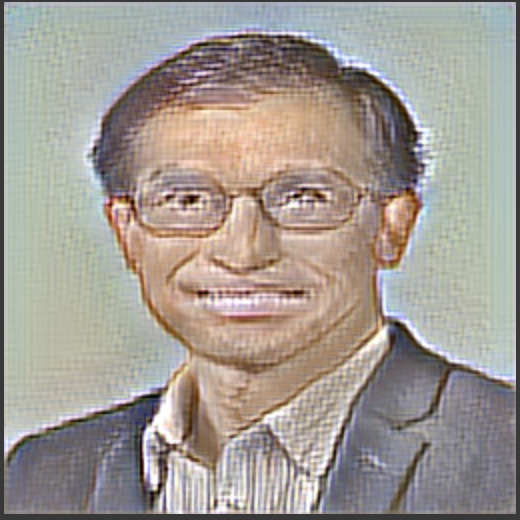
\includegraphics[width=0.3\textwidth]{figures/1.png}
			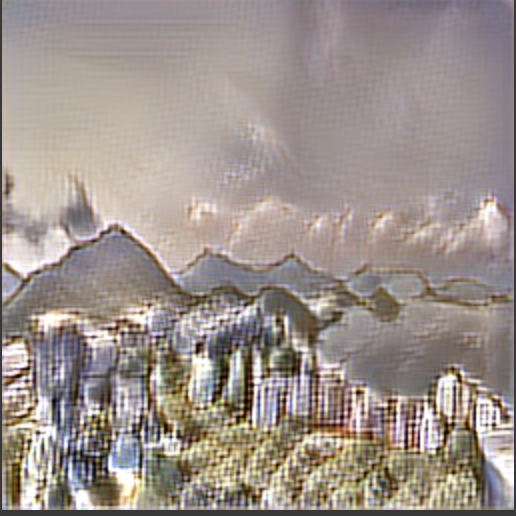
\includegraphics[width=0.3\textwidth]{figures/2.png}
			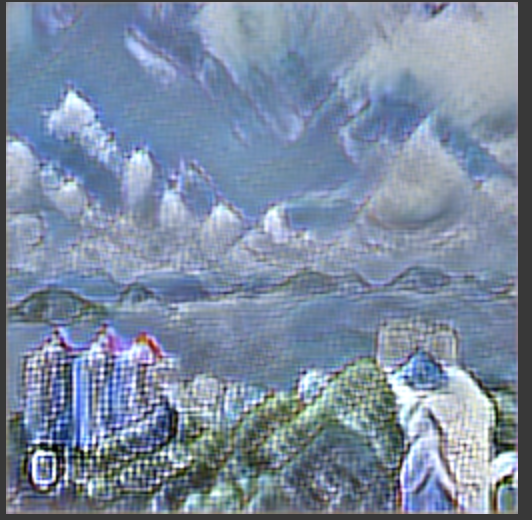
\includegraphics[width=0.3\textwidth]{figures/3.png}
		\end{figure}
		The left two images capture early renaissance painting style and apply it to Prof. Yeung and HKUST image. The rightmost image captures the starry night style and combine it with HKUST image.
	\item[Q9] The training distribution is given in the table below:
		\begin{center}
			\begin{tabular}{|c|c|c|c|c|c|c|c|}
				\hline
					& dog &  elephant &  giraffe &  guitar & horse &  house &  person \\
				\hline
				art painting &   13 &        13 &      231 &      10 &    180 &     11 &      11 \\
				\hline
				cartoon      &  10 &        13 &       12 &     121 &     11 &     12 &      12 \\
				\hline
				photo        &  10 &       13 &       12 &      10 &     11 &    215 &     211 \\
				\hline
				sketch       & 229 &     217  &     10   &    9 &     8 &     13 &      13 \\
				\hline
			\end{tabular}
		\end{center}
		The test distribution is given in the table below:
		\begin{center}
			\begin{tabular}{|c|c|c|c|c|c|c|c|}
				\hline
					 &   dog & elephant & giraffe & guitar & horse & house & person \\
					 \hline
				art painting & 119 &      89 &      110 &      82 &     90 &    110 &     96 \\
				\hline
				cartoon &       95 &        83 &      109 &      82 &     81 &   101 &      95 \\
				\hline
				photo &         81 &        83 &      102 &      81 &   103 &     95 &     110 \\
				\hline
				sketch  &      112 &       115 &      104 &      95 &    108 &     80 &     112 \\
				\hline	
			\end{tabular}
		\end{center}
		In the training distribution, the data is very unbalanced. For example, the majority of sketch are either dog and elephant. 

		In the test distribution, the data is relatively balanced, having an even number of data in each cell in the table.
	\item[Q10] It is expected that the classifier will learn the unbalanced distribution in the training set. Therefore, for data that belongs to the sketch category, most of them are dogs or elephants. Hence, the classifier may classify most sketches as dogs and elephants, creating false positive for dogs and elephants and false negative for other data in the sketch category.
	\item[Q11] The number of trainable parameters is $5619804$.
	\item[Q12] The cross entropy loss at the end is $0.014$
	\item[Q13] For training dataset, the accuracy is around 95 percent. However, for the test set, the accuracy is around 42.1 percent which is much lower. The confusion matrix in the training set is given by:
		\begin{verbatim}
			[[222  24   0   0   5   2   1]
			[  3 246   0   0   1   0   0]
			[  9   0 252   0   1   0   0]
			[  1   0   1 138   5   0   0]
			[  5   0   2   0 193   0   1]
			[  1   2   0   0   0 242   0]
			[  4   1   0   0   0   0 238]]
		\end{verbatim}
		while that in the test set is given by:
		\begin{verbatim}
			[[110  58  42  28 120  14  29]
			[ 57 157  40   4  81  11  17]
			[ 76  32 202  22  57  19  12]
			[ 48  20  49 138  50  14  18]
			[ 77  52  23  31 162  11  16]
			[ 16  21  52  15  61 214   6]
			[ 35  46  24  20  90  23 168]]
		\end{verbatim}
	\item[Q14] Here are some misclassified image
		\begin{figure}[H]
			\centering
			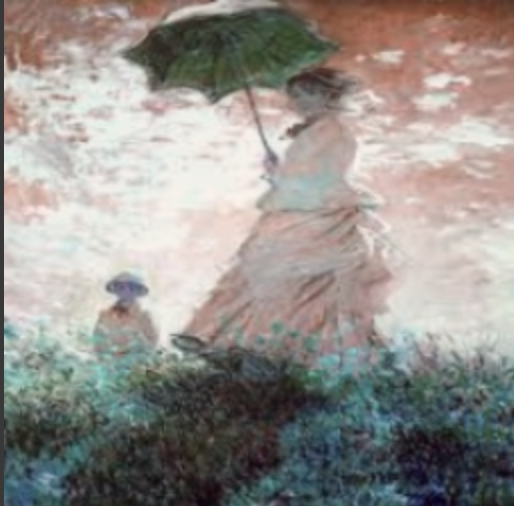
\includegraphics[width=0.5\textwidth]{figures/4.png}
		\end{figure}
		This is classified as elephant while it should be a person. This photo belongs to art painting category. This may be because a lack of art painting category for person.
		\begin{figure}[H]
			\centering
			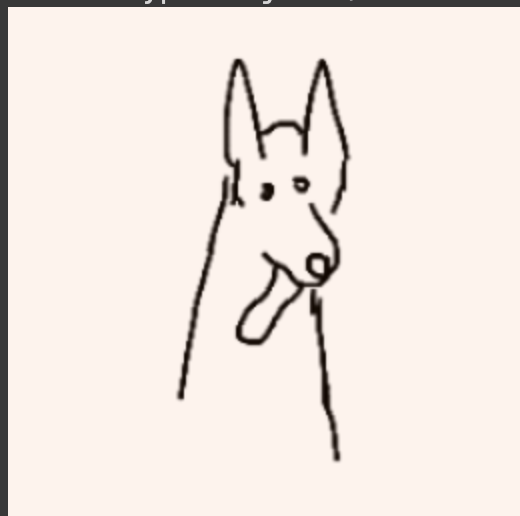
\includegraphics[width=0.5\textwidth]{figures/5.png}
		\end{figure}
		This is classified as elephant again while it should be a dog. This photo belongs to the sketch category. This misclassification may be because there are a lot of sketches for dogs.
	\item[Q15] Here are some samples of generated dataset
		\begin{figure}[H]
			\centering
			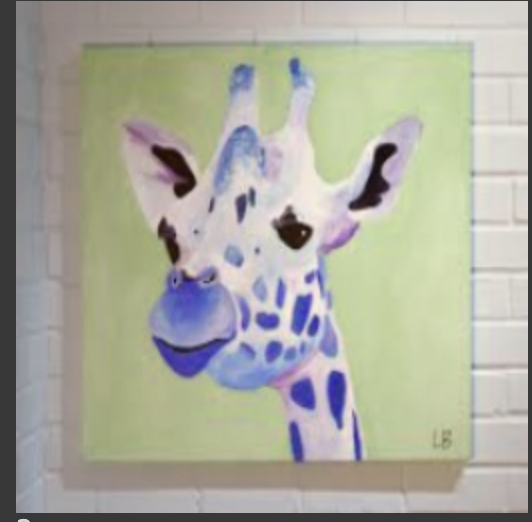
\includegraphics[width=0.3\textwidth]{figures/7.png}
			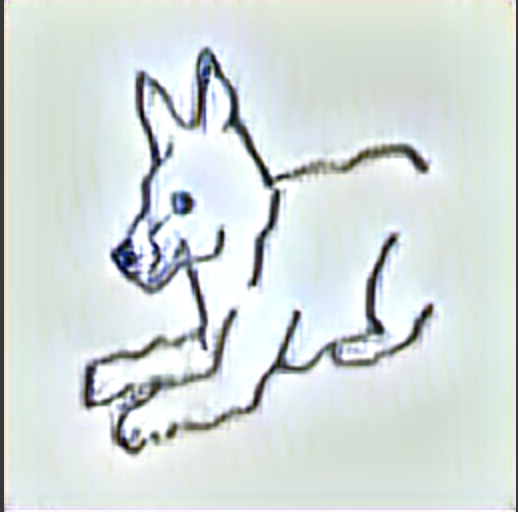
\includegraphics[width=0.3\textwidth]{figures/8.png}
		\end{figure}
	\item[Q16] The cross entropy loss after training on the augmented dataset is $0.23$.
	\item[Q17] The accuracy on the test set becomes $0.44$.
		The confusion table is given below:
		\begin{verbatim}
			[[ 81  87  83  25  87  18  21]
			[ 25 169  72   8  61  14  19]
			[ 75  28 233  12  31  31   8]
			[ 46  10  32 177  37   7  25]
			[ 66  61  33  31 143  24  20]
			[ 16  47  79  18  21 187  12]
			[ 27  28  73  24  45   7 204]]
		\end{verbatim}
		which is slightly better than before.
	\item[Q18] The augmentation provides some rare data that is not present in the original dataset. This avoids biases in the model. The augmentation also increases the size of the dataset. Hence, the model can learn better.

\end{enumerate}
\end{document}
